\chapter{Discussion}
\label{ch:discussion}

Aimed at contributing to the research on the question of integration of allothetic and idiothetic information at the level of the hippocampal place cells, I used freely-moving virtual reality setup where I conducted several types of electrophysiological experiments with randomly foraging animals. To study the place cell spatial representation I designed vSHIFT, vGAIN and vTELEPORT experiments, each implementing a mismatch between the boundary-defined and the visual reference frames.

From the vSHIFT - coherent experiment we learn that most of the CA1 place cells are getting self-motion inputs. The analysis of the place field shift in the conflicting sensory conditions showed simultaneous encoding of both reference frames, balanced from mostly self-motion driven near the boundaries to the visually driven in the center of the arena. Analysis of the interplay between the visual and self-motion inputs in the vSHIFT experiment confirms better position calibration in the presence of the boundaries versus to the middle of the arena. It was found that, despite previous suggestions that CA1 cells responsive to visual and self-motion cues are anatomically separated (\cite{Fattahi2018}), an evidence that the same CA1 cell can integrate both types of self-motion and visual inputs on the single cell level. These CA1 cells can not only be visually or self-motion selective, but also represent a specific combination of the two types of inputs - forming distinct categories of place fields. Current experiments demonstrate that place cells having self-motion components in their place fields keep being driven by self-motion inputs only, if the visual component is not available. This suggests place cells could use weighted integration of allocentric and idiothetic sensory afferents for spatial encoding.

In the vGAIN experiment, sessions with animals recorded with the 1.2x gain condition showed the strong ability of the hippocampal cells to encode both visual and boundary-defined reference frames even during and after being in conflict between the proprioceptive and visual systems. The distribution of the place fields shifts shows a substantial amount of units having shifts of 0m (visually-driven fields) and 0.3m (boundary driven fields), similar to the regular physical or visual shift experiment. An outstanding amount of fields with the place field shift of 0.15m confirms the above hypothesis of an ability of the hippocampus to represent location as a combination of visual-landmark- and boundary-defined reference frames. Recordings in dark allowed to show that the induced visual- to self-motion conflict results in recalibration of the overall spatial representation, possibly via feedback projections from the hippocampus to the entorhinal cortical areas.

While we collected evidence from both vSHIFT and vGAIN 1.2x experiments that under small conflicts place cells tend to integrate both sensory inputs, the vGAIN 1.4x suggests that in a situation of a larger conflict one sensory modality is being abandoned. Moreover, in line with previous human and animal studies (\cite{Zhao2015}; \cite{Shettleworth2005}), we found that in larger conflicts involving vision path integration tend to be implemented based on non-visual (mostly self-motion, but can be also tactile and olfactory) sensory inputs only; cells mostly encode positions relative to the environmental boundaries, ignoring information coming from vision.


\section{Integration of the self-motion and visual information}
\label{sec:integration_sm_vision}

It is established that hippocampal cells can build spatial representations without self-motion inputs - mainly the grid cell inputs from the entorhinal cortex (\cite{Poucet2015}; \cite{Muessig2015}). Moreover, without the stable grid cell activity new place cells can be established in new environments (\cite{Brandon2014}). This leads to an assumption that both external sensory and internally-generated self-motion information come to the hippocampus as two different, potentially overlapping, parallel pathways - one integrating proprioceptive, vestibular and other idiothetic signals to represent self-motion, another providing a combination of the allocentric sensory signals instantaneously occurring at a particular location.

The data from current experiments demonstrates the reliance of place cells on these inputs via encoding position based either on self-motion, or on visual information, or on combination of both (see results). In contrast to the identified groups of neurons recorded in the body-fixed VR (\cite{Haas2019}), where a negligible subset of neurons shows integrative properties of both allothetic and idiothetic (proprioceptive) inputs, we found a large subset of hippocampal cells being selective based on both types of input. This suggests there is an interference between two input pathways, and involvement of some competitive learning mechanisms used by the hippocampal CA1 neurons to establish their firing preference based on one or another information stream, or a combination of them. This in turn, would suggest a much stronger contribution of self-motion-driven path integration to hippocampal spatial representation than what could be expected from head- or body-fixed VR experiments (\cite{Jayakumar2018}; \cite{Haas2019}; \cite{Chen2013}, \cite{Aronov2014}).

Also, it was long assumed that in absence of boundary-defined reference frame, additional allocentric (e.g. visual) information can “reset” the path integrator, which should move the place field centers such that they have 0m shift and belong to the “visual” group, to represent the position defined solely by the allocentric frame (\cite{Savelli2008}). Instead, our data shows that the information about the moved distance is somehow integrated in the pre-hippocampal brain circuits to represent the average between the distances defined by two different reference frames, and does not simply bind to one or another, at least at small conflicts (see results about removal of a visual reference frame).


\section{Representation of a combination of different reference frames}
\label{sec:integration_two_frames}

Clear effect of visual influence on multisensory boundary-and-visual cells shows that the pure boundary vector cell model (\cite{Barry2006}; \cite{Grieves2018}) or different periodic grid cells inputs (\cite{OKeefe2005}; \cite{Rolls2006}) is not highly probable. The recent work involving single-cell recordings, where place fields can be induced by precise time stimulation (\cite{Zhao2020}), demonstrates that co-firing, or general synaptic plasticity should be a mechanism for recruitment of particular CA1 cells to integrate visual, boundary or multimodal inputs and form a field of a certain type. Another work shows that dendritic plateau potentials, coming from the EC3 in conjunction with CA3, are sufficient to produce place field in CA1 pyramidal cells by means of strengthening synaptic inputs active around the time of plateau formation (\cite{Bittner2015}). Altogether this is a strong evidence for the crucial role of synaptic plasticity in integration of allothetic and idiothetic inputs. Below I would like to propose a few mechanisms how it could be involved in the process of coding an intermediate estimate of the positions, defined by two reference frames.


\subsection{Effect of a shift of a particular reference frame after learning and establishing a place field}

One possible explanation how the average between visual- and boundary-defined distances could be implemented by the hippocampal neurons would be to assume that pyramidal cells, having these fields, receive both inputs from the self-motion (distance from arena walls) and visual (distance to proximal virtual cues) streams. At the time of original field formation, the corresponding sensory and path integrator signals are coherently coming as inputs to the pyramidal neurons to form a stable place field, defined by mutual presence of information about the distance to the walls and information about visual landmarks. This could be done by strengthening the necessary synaptic connections between the appropriate sensory afferents and a particular post-synaptic neuron, encoding this place field. In the shifted condition, signals from the path integrator and a visual system might loose their coherence and appear to be shifted relative to each other in space (Figure 37), leading to the asynchrony in the incoming cell firing and to a shift of the place field center to a half distance between the original position and actual arena shift. If this is the case, this would lead to different place field characteristics between the original and the shifted conditions. If incoming signals are not coherent and have only partial overlap, this should decrease the place field peak firing rate in case of the additive synapses. Also the place field should appear to be larger, as one of the inputs starts to be active earlier (later).

\begin{figure}
\captionsetup{format=plain}
\makebox[\textwidth]{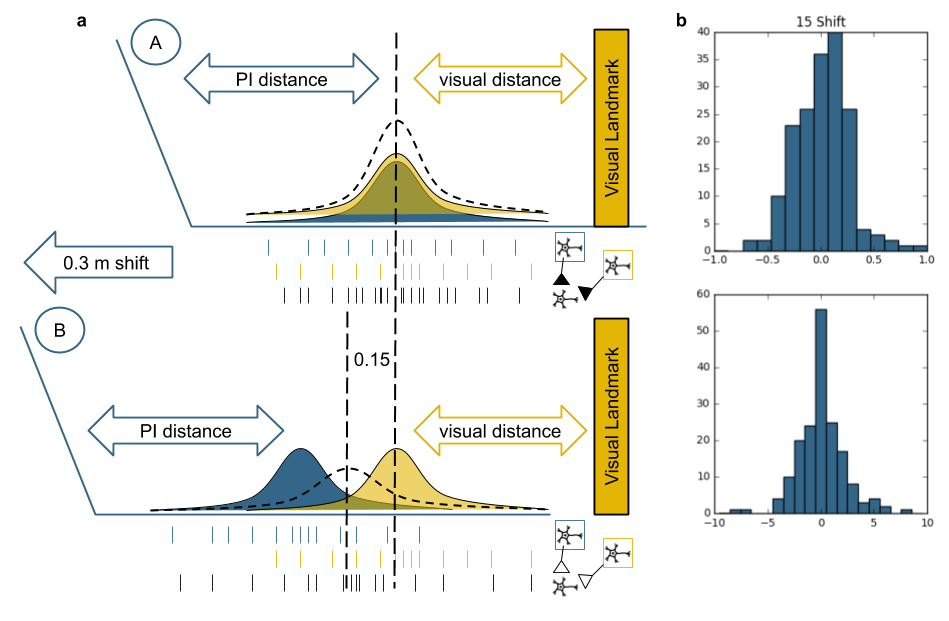
\includegraphics[width=150mm]{figures/F37_encoding_average.png}}
\caption[Encoding average]{
Weighted integration of visual and self-motion inputs might lead to the average representation of the resulting position estimate. (a) Schematic of the inputs to the postsynaptic CA1 neuron. Visual (yellow) and self-motion (blue) afferent estimations are learned in a coherent representation by some CA1 neuron (top row). In a conflicting situation incoming inputs are not aligned which can lead to the averaging of the inputs if the cell is using weighted input integration. Applicable if the conflict is small (place fields overlap). (b) No change in mean firing rate (top plot) and field size (bottom plot) between original and shifted (conflicting) conditions for the group of cells showing average position encoding.
}
\label{fig:F37_encoding_average}
\end{figure}

I verified whether on average place fields in this middle group (0.15m place field shit +- 1 SD of 0.082m) change their firing characteristics between two conditions. Although some of the cells demonstrate exactly these effects (not shown), the total majority of the fields in this group keep their firing rate and field size stable between original and shifted conditions (see Figure 37b). This suggests that either the synaptic connections are multiplicative, or in general there is another mechanism how the average location between points in two reference frames can be represented. One of the opportunities for further investigations is to use the advantage of the VR system and record these groups of cells’ activity when first one and then the other inputs are completely removed.


\subsection{Change in input reliability together with Bayesian coding may explain categorization of CA1 cells by input preference}

According to the principles of optimal Bayesian coding (\cite{Pouget2003}) the weighted integration of sensory estimates should have weights proportional to the reliability of the estimate, in order to maximize the resulting estimate. Intuitively, the reliability of the position estimation relative to the boundaries is highest near the walls (supported by tactile contact) and lowest in the arena center. At the same time position estimation relative to both proximal and distal visual cues and landmarks is almost the same everywhere in the arena except at the actual arena walls, where the quality of the projection is low. If CA1 neurons use weighted integration, having these assumptions a Bayesian estimations integration model (like used in the seminal study by \cite{Ernst2002}) can explain the continuous distribution of place field shifts recorded in the vSHIFT experiments (Figure 38).

\begin{figure}
\captionsetup{format=plain}
\makebox[\textwidth]{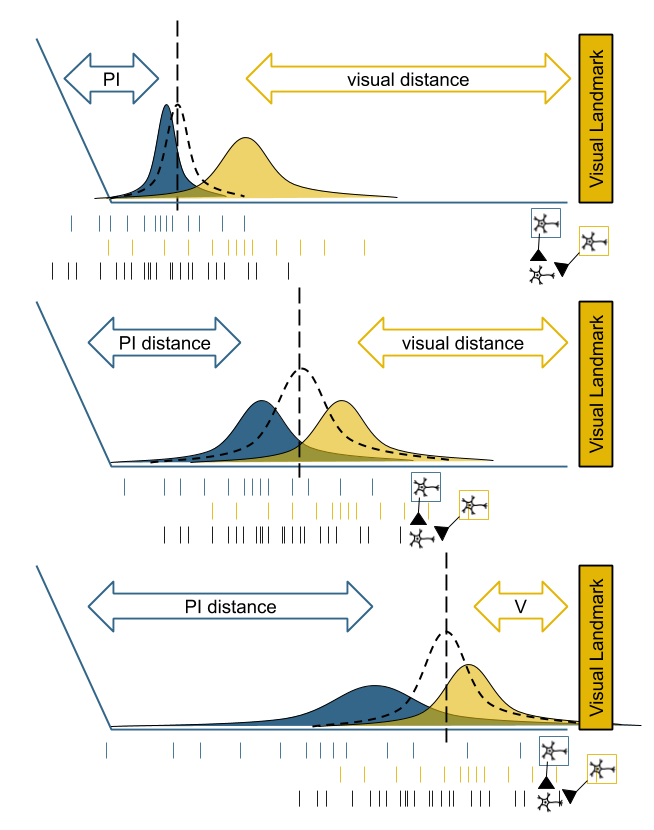
\includegraphics[width=100mm]{figures/F38_weighted_integration.png}}
\caption[Weighted integration]{
Conflicting presynaptic inputs in different places within the arena together with Bayesian coding can lead to formation of all categories of visually and self-motion driven place cells. (top) High reliability of the self-motion inputs near the boundaries results in formation of self-motion driven place cells. (middle) Relatively equal contribution of both types of sensory inputs leads to formation of cells encoding average between reference frames. (bottom) Higher reliability of the visual signals away from the boundaries results in formation of visually-driven place cells.
}
\label{fig:F38_weighted_integration}
\end{figure}

In particular, one can assume that indirect EC2 inputs to the hippocampus e.g. to the area CA3 might lead to the existence of two different continuous attractor networks, each encoding position relative to a different reference frame (\cite{Li2020}, \cite{Haas2019}). Then instead of classifying CA1 cells in different groups we hypothesize all cells use the same principles of sensory integration (near-like optimal), with the difference that some cells initially by chance are more strongly connected (e.g. via schaffer collaterals) with the neurons from the attractor encoding position based on self-motion, and some with the attractor encoding position based on visual inputs. This assumption can also explain why there is a balance in favor of vision in the middle of the arena, while there is a clean domination of the position encoding relative to the boundaries near arena walls (see results).


\subsection{Frequent arena shift results in encoding intermediate position by accumulation of synaptic plasticity effect}

Another option how a place field could shift to a half distance between estimates is when it is assumed that those self-motion and visual inputs, that have maximum cumulative probability of simultaneous firing among both original and shifted conditions, are integrated (Figure 39a). Assuming a cell has a stable visual input relative to a certain visual landmark, it could be that the chances of integrating the self-motion input that has maximum firing probability in both original and shifted are the highest, leading to a place field that shifts by a half distance of the arena shift (Figure 39a).

\begin{figure}
\captionsetup{format=plain}
\makebox[\textwidth]{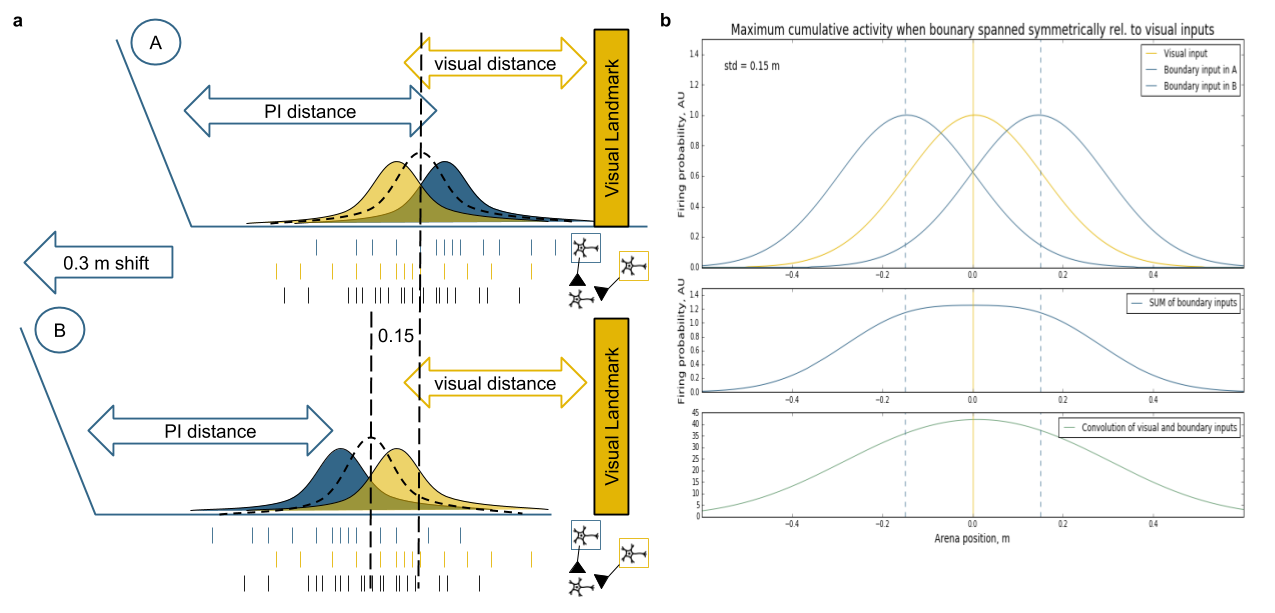
\includegraphics[width=150mm]{figures/F39_symmetric_encoding.png}}
\caption[Symmetric encoding]{
Symmetric positioning of self-motion inputs around visual input can lead to an average encoding. (a) When position relative to both reference frames is always in conflict, the higher probability of mutual spiking will happen to sensory afferents shifted 0.15m relative to each other in both conditions. (b) In cases of small conflicts the convolution of the putative visual and self-motion place afferents is highest when they are shifted 0.15m relative to each other like in (a).
}
\label{fig:F39_symmetric_encoding}
\end{figure}

Assuming all inputs do have regular gaussian spiking probability, this could be confirmed by computing the convolution between the stable visual input and both self-motion driven inputs in both conditions, located 0.3m apart from each other. If place field sizes relative to the longitudinal arena shift are large enough, the maximum convolution will be when the visual input is located symmetrically between self-motion inputs (in our case an average field size of 0.4m, Figure 39b) Even if the two original and shifted conditions never appear at the same time, some potential accumulation of the total mutual spiking of these visual and symmetrically located self-motion inputs and a postsynaptic neuron can lead to an increased connection by hebbian plasticity, resulting in this half-distance situation.


\subsection{Behavior of multisensory cells can be explained by dynamic loops in the hippocampal-entorhinal network}

However, the actual mechanisms could be more complicated. A recent modelling work of a entorhinal-hippocampal system, assuming necessary involvement of recurrent connections from the CA1 to the EC region (\cite{Li2020}), can explain the half-distance shift phenomena. The dynamic loop-based network model, tested against the multi-compartment experimental data (\cite{Carpenter2015}; \cite{Wernle2018}), demonstrates the same effect on the level of CA1 place cells when self-motion and visual cues are in conflict. Authors performed a simulation of the condition with gain between the vision and self-motion in a similar rectangular arena-like experiment, and found that the population of place cells shifts to the intermediate position between the self-motion and visual estimates. This effect is explained by the dynamic loop-like interaction between the visually-driven place cells and populations of grid cells, which are shifted by them towards the visually identified location. To verify this hypothesis a more precisely defined gain experiment can be designed and implemented.


\section{Aspects of using freely-moving virtual reality system}
\label{sec:aspects_of_vr}

The use of the freely-moving virtual reality system has its advantages but also potential drawbacks. As all conventional virtual reality systems, ratCAVE is an excellent instrument for visual manipulations and induction of a visual to movement mismatch, in a closed-loop with the computation of the animal position. The freely-moving condition is far more naturalistic compared to the head or body fixed conditions, where certain internal (vestibular, proprioceptive) and external (feeling of boundaries) information is not present. It also allows for easier and shorter training protocols (\cite{Ferreiro2020}) avoiding any animal fear states.

The existence of boundaries might be of a special importance as the boundary driven cells have significant impact on the place code (\cite{Okeefe1996}; \cite{Barry2006}; \cite{Savelli2008}). Environmental boundaries play a special role in the formation of a spatial map, without physical contact with the walls, as it is usually in conventional virtual reality systems, the map of space at the level of place cells might not be complete.

However, the same issue can be applied to the ratCAVE. The 3D virtual reality setup allows placing 3D virtual objects inside the arena, not just having visual proximal or unreachable distal landmarks on the walls. Although this makes the virtual environment more immersive, absence of the physical tactile contact with virtual objects might affect their representation in the brain, potentially reducing their significance for the spatial map. In particular, object vector cells (\cite{Hooydal2019}), which play an important role in spatial coding, might be affected. Favourably, current experimental results demonstrate strong influence of the visual cues on the hippocampal place cells, so the overall influence of visual virtual objects is doubtless - however the amount of the mismatch between visual object appearance and their tactile insensitivity is to be identified.


\section{Aspects of experimental design}
\label{sec:aspects_of_design}

I recorded several sessions of the shift and gain experiments with the same cohort of animals. Theoretically, this might bias the experimental data in a few ways.

First, after several sessions being in the same experimental protocol, animals can better learn the environment and understand that the projected visual reference frame is not required to get food rewards. This might influence the amount of visual place encoding down to complete ignorance of the virtual reference frame. To account for that, tests for the difference in the amount of visually or self-motion selective cells across days were done. They do not show any difference.

Second, some animals were used in both shift and gain experiment types. Hypothetically, the knowledge of one virtual environment may influence the behavior of cells in another condition - as both virtual shift and gain environments are the same, the knowledge of the environment in one condition (e.g. shift) might cause activation of the same cells in another condition (e.g. gain), which would not happen otherwise due to, for instance, ignorance of the visual flow because of the proprioceptive mismatch. To be sure to exclude this influence, experiments with separated cohorts of animals should be performed.


\section{Open questions}
\label{sec:open_questions}

It is still not clear at which stage the integration of the self-motion and external sensory information is done. One possibility for the multisensory neurons would be to integrate recurrent inputs from the same CA1 - CA3 circuit, basically working with the same visually- and boundary-defined cells in CA1. Another possibility would be to get direct self-motion and sensory inputs from the mEC / lEC. An opportunity to test these options would be to perturb entorhinal inputs to the hippocampus while recording the shift experiment and investigate the change of activity of the multisensory neurons.

Apart from that, data showing the integration of the inputs on the hippocampal level confirms the idea of a hippocampus as a general memory device - providing mechanisms to match and update neuronal firing patterns representing recurrently occuring episodes, that allows to implement stable place fields, like any memory sharpens and stabilizes with repeats. Further design of experimental protocols with gradual visual virtual cue manipulations could provide more insights into the mechanisms of pattern completion and pattern separation - investigating the stability of the recorded place fields, or a change in the place field firing depending on the changes in the virtual environment.
